
\section{Descriptions des besoins}

\subsection{Besoins Fonctionnels}
\subsubsection{Plateau de Jeu}

\begin{center}
    \centering
    \begin{tabular}[h]{|m{14cm}|m{2cm}|} 
    \hline
    \rowcolor[HTML]{FFA8A8}
    \multicolumn{2}{|c|}{\textbf{Priorité 3/3}}\\
    \hline
    Besoins & Avancement\\
    \hline
    • Les hexagones numérotés, chacun représentant une distance définie, par défaut : 16 kilomètres & \FAIT \\ 
    • Définir les joueurs et leurs spécificités. Par exemple les nationalités possibles, le joueur qui joue le premier et celui qui a l’initiative. & \FAIT \\
    • Pouvoir poser des unités sur la carte et à retenir celles qui ne sont pas présentes dans celles-ci & \FAIT \\
    • Pouvoir poser plusieurs unités sur un hexagone & \FAIT \\
    • Définir une séquence de tour : 
    \begin{itemize}
        \item Pouvoir alterner entre les joueurs
        \item Respecter l’ordre strict d’un tour
    \end{itemize} 
    & \FAIT \\
    • Afficher un terminal qui permettra aux joueurs de donner des commandes d'attaque ou mouvement & \FAIT \\
    • Être capable de faire des lancés de dés et d’appliquer des modificateurs. La majeure partie du jeu se base sur les dés & \NOP \\
    • Pouvoir déterminer quel joueur a l’initiative & \NOP \\
    \hline
    \end{tabular}
\end{center}

\begin{center}
    \centering
    \begin{tabular}[h]{|m{14cm}|m{2cm}|} 
    \hline
    \rowcolor[HTML]{FFB72B}
    \multicolumn{2}{|c|}{\textbf{Priorité 2/3}}\\
    \hline
    Besoins & Avancement\\
    \hline
    • Différencier plusieurs types de terrain, les montages, les mers de sable et les crêtes par exemple & \FAIT \\
    • Créer une base pour les cartes d’évènements. Celles-ci étant très différentes, l’implémentation sera limitée aux évènements génériques (non spécifiques aux scénarios) & \FAIT \\
    • Pouvoir charger la carte du jeu à partir d’un fichier \textsc{txt} ou \textsc{json} et pouvoir la sauvegarder aux mêmes formats & \FAIT \\
    \hline
    \end{tabular}
\end{center}

\begin{center}
    \centering
    \begin{tabular}[h]{|m{14cm}|m{2cm}|} 
    \hline
    \rowcolor[HTML]{C0D8C0}
    \multicolumn{2}{|c|}{\textbf{Priorité 1/3}}\\
    \hline
    Besoins & Avancement\\
    \hline
    • Ajouter les différents types d’indicateurs afin d’illustrer les villages, les villes et les oasis par exemple & \FAIT \\
    \hline
    \end{tabular}
\end{center}
 
\subsubsection{API}

\begin{center}
    \centering
    \begin{tabular}[h]{|m{14cm}|m{2cm}|} 
    \hline
    \rowcolor[HTML]{FFA8A8}
    \multicolumn{2}{|c|}{\textbf{Priorité 3/3}}\\
    \hline
    Besoins & Avancement\\
    \hline
    • Pouvoir échanger des informations basiques entre serveur et client & \FAIT \\ 
    • Pouvoir convertir un état de la carte du jeu en format utilisable par le client pour pouvoir ensuite afficher le plateau & \FAIT \\
    • Envoyer un coup joue dans un format utile pour le serveur, pour pouvoir faire des éventuelles modifications sur le plateau & \FAIT \\
    • Vérification des coups : 
    \begin{itemize}
        \item Envoyer le coup joue au serveur
        \item Vérifier que le coup est valide
        \item Retourner une réponse positive ou négative. Si le coup est bon alors envoyer le nouvel état de la carte du jeu au client
    \end{itemize} 
    & \FAIT \\
    \hline
    \end{tabular}
\end{center}

\subsubsection{Unités}

\begin{center}
    \centering
    \begin{tabular}[h]{|m{14cm}|m{2cm}|} 
    \hline
    \rowcolor[HTML]{FFA8A8}
    \multicolumn{2}{|c|}{\textbf{Priorité 3/3}}\\
    \hline
    Besoins & Avancement\\
    \hline
    • Définir l'unité comme interface, qui aura une morale, peut être perturbée (disrupted) et qui peut prendre des actions basiques comme attaquer et bouger & \FAIT \\ 
    • Implémenter le système similaire à des points de vie (voir partie \textit{Depletion} des règles)  & \FAIT \\
    • Séparer les unités en catégories différentes : motorisées, à pied, mécanisées, cavalerie... & \FAIT \\
    • Mettre en place les situations ou l'unité devient perturbée : 
    \begin{itemize}
        \item Trop de troupes sur un hexagone
        \item Fin d'un mouvement de nuit
        \item Après la phase de \textit{Supply Attrition}, il y a un échec sur le test d'usure (attrition)
    \end{itemize} 
    & \FAIT \\
    \hline
    \end{tabular}
\end{center}

\begin{center}
    \centering
    \begin{tabular}[h]{|m{14cm}|m{2cm}|} 
    \hline
    \rowcolor[HTML]{FFB72B}
    \multicolumn{2}{|c|}{\textbf{Priorité 2/3}}\\
    \hline
    Besoins & Avancement\\
    \hline
    • Permettre aux unités éligibles de s'entraîner et de faire des améliorations & \NOP \\
    \hline
    \end{tabular}
\end{center}

% \subsubsection{Organisation de l'armée}


\subsubsection{Mouvement}

\begin{center}
    \centering
    \begin{tabular}[h]{|m{14cm}|m{2cm}|} 
    \hline
    \rowcolor[HTML]{FFA8A8}
    \multicolumn{2}{|c|}{\textbf{Priorité 3/3}}\\
    \hline
    Besoins & Avancement\\
    \hline
    • Déplacement case par case et enlever les points de mouvement correspondants de l'unité. Ceci pour limiter la capacité de mouvement & \FAIT \\
    • Le joueur du Commonwealth peut accélérer le mouvement de ses unités en utilisant le rail et transport maritime & \NOP \\
    \hline
    \end{tabular}
\end{center}

\begin{center}
    \centering
    \begin{tabular}[h]{|m{14cm}|m{2cm}|} 
    \hline
    \rowcolor[HTML]{FFB72B}
    \multicolumn{2}{|c|}{\textbf{Priorité 2/3}}\\
    \hline
    Besoins & Avancement\\
    \hline
    • Déplacement d'un point A à un point B, en parcourant le plus cours chemin. On utilisera l'algorithme \emph{Dijkstra} pour satisfaire la condition & \FAIT \\
    • Appliquer un bonus de mouvement dépendant du terrain d'un hexagone. C'est plus facile de se déplacer sur une plaine plutôt qu'à travers des montagnes & ? \\
    • Permettre aux unités qui doivent se replier de bouger de 1-3 hexagones. Ce mouvement ne coûte pas de points de mouvement & \FAIT \\
    • Ajouter la mécanique du \emph{overrun} (fuite). Les unités capables de le faire peuvent pendant leur phase de mouvement attaquer des unités. Les défenseurs alors peuvent utiliser leurs phases de réaction pour bouger un certain nombre d'hexagones. La distance est définie par l'unité concernée & \NOP \\
    \hline
    \end{tabular}
\end{center}

\begin{center}
    \centering
    \begin{tabular}[h]{|m{14cm}|m{2cm}|} 
    \hline
    \rowcolor[HTML]{C0D8C0}
    \multicolumn{2}{|c|}{\textbf{Priorité 1/3}}\\
    \hline
    Besoins & Avancement\\
    \hline
    • Mouvement la nuit & \FAIT \\
    \hline
    \end{tabular}
\end{center}

\subsubsection{Combat}

\begin{center}
    \centering
    \begin{tabular}[h]{|m{14cm}|m{2cm}|} 
    \hline
    \rowcolor[HTML]{FFA8A8}
    \multicolumn{2}{|c|}{\textbf{Priorité 3/3}}\\
    \hline
    Besoins & Avancement\\
    \hline
    • Pouvoir définir les unités participant au combat de ce round & ? \\
    • Pouvoir déterminer la puissance de combat de l'armée composée de ces unités & ? \\
    • Définir les règles du combat, par exemple le fait que seules les unités/armées adjacentes peuvent entrer en combat, par la volonté de l'attaquant & ? \\
    • Pouvoir simuler le combat et donner les résultats :
    \begin{itemize}
        \item Déterminer les dégâts causés par une unité en divisant les points d'attaque par les points de défense de l'ennemie pour obtenir un ratio.
        \item Séparer les défenseurs en groupe de morale. Les unités avec la même morale se retrouvent dans le même groupe. Les résultats seront dans l'ordre descendant de morale. Par exemple si on a deux groupes de morale (de 1 et 2), alors les résultats du combat seront d'abord appliqués dans le groupe avec une morale de 2, puis a celui de morale 1.
        \item Appliquer des éventuelles règles spéciales.
        \item Si un hexagone contient que des unités de support, alors lancer un dé si l'attaquant le souhaite, pour tenter de capturer les unités.\newline Un résultat de 1-3 est un succès et un résultat de 4-6 veut dire que les unités de support sont détruites.
        \item Amasser les dégâts et puis causer des dégâts aux unités adverses.\newline Les dégâts sont divis jusqu'à que le maximum d'unités ait reçu un point de dégât, puis infliger les deuxièmes points de dégâts sur les unités, s'il reste des points de dégâts à distribuer.
        \item Enlever du plateau les unités détruites, et les ajouter dans la liste d'unités détruites du joueur concernée.
        \item Lancer un dé pour faire le test de morale des unités qui reste. Si le test échoue, alors l'unité est \"disrupted\".
    \end{itemize} & ? \\
    • Pouvoir simuler la retraite d'une armée si les spécifications le permettent, par exemple le terrain et la condition de l'armée est convenable, et si l'utilisateur le souhaite & ? \\
    \hline
    \end{tabular}
\end{center}

\begin{center}
    \centering
    \begin{tabular}[h]{|m{14cm}|m{2cm}|} 
    \hline
    \rowcolor[HTML]{C0D8C0}
    \multicolumn{2}{|c|}{\textbf{Priorité 1/3}}\\
    \hline
    Besoins & Avancement\\
    \hline
    • Si un Hex contient plusieurs terrains, le défendant doit pouvoir en choisir un pour sa défense & ? \\
    \hline
    \end{tabular}
\end{center}

\subsubsection{Opérations Aériennes et Navales}

\begin{center}
    \centering
    \begin{tabular}[h]{|m{14cm}|m{2cm}|} 
    \hline
    \rowcolor[HTML]{C0D8C0}
    \multicolumn{2}{|c|}{\textbf{Priorité 1/3}}\\
    \hline
    Besoins & Avancement\\
    \hline
    • Pouvoir déterminer les différentes unités aériennes et navales ainsi que leurs spécificités & \FAIT \\
    • Pouvoir déterminer les différentes cibles, par exemple des bases militaires ou les rivages(pour les opérations navales surtout), qu'ils peuvent cibler et attaquer & \FAIT \\
    • En ce qui concerne les opérations navales, ils peuvent effectuer des expéditions transportant des munitions ainsi que des unités/machines de guerre & \FAIT \\
    \hline
    \end{tabular}
\end{center}

\subsubsection{Affichage}

\begin{center}
    \centering
    \begin{tabular}[h]{|m{14cm}|m{2cm}|} 
    \hline
    \rowcolor[HTML]{FFA8A8}
    \multicolumn{2}{|c|}{\textbf{Priorité 3/3}}\\
    \hline
    Besoins & Avancement\\
    \hline
    • Afficher le joueur dont c'est le tour & \FAIT \\
    • Déterminer et afficher les informations de fin de partie et du vainqueur & \FAIT \\
    • Afficher les différents marqueurs sur l'état de chaque composante du jeu, par exemple hors d'approvisionnement pour les unités & \FAIT \\
    • Afficher le résultat et les informations à la fin du combat & \FAIT \\
    \hline
    \end{tabular}
\end{center}

\subsubsection{Réseaux}

\begin{center}
    \centering
    \begin{tabular}[h]{|m{14cm}|m{2cm}|} 
    \hline
    \rowcolor[HTML]{FFA8A8}
    \multicolumn{2}{|c|}{\textbf{Priorité 3/3}}\\
    \hline
    Besoins & Avancement\\
    \hline
    • Le jeu sera autour d'une architecture client-serveur qui puisse se déployer à travers Internet (pas seulement sur un réseau local) & \FAIT \\
    \hline
    \end{tabular}
\end{center}

\subsection{Besoins Non-Fonctionnels}

\subsubsection{Affichage}
\begin{itemize}
    \item Affiche un message d'erreur ou de refus quand une requête ou commande invalide est entrée.
    \item Mettre en place une interface graphique affichant le plateau du jeu, les unités.
    \item Afficher un message d'attente au joueur  qui ne joue pas .
\end{itemize}

\subsubsection{Système}
\begin{itemize}
    \item Le temps d'attente entre un coup proposé et sa validité évalué devront être de l'ordre de la seconde.
    \item Un chat sera créé pour communiquer avec l'adversaire.
\end{itemize}

\section{Scénario}

Les joueurs devront se connecter sur un serveur afin d'accéder à la partie. Le serveur hébergera la partie en traitant les mécanismes de la partie en arrière-plan. Les utilisateurs recevront une interface graphique en provenance du serveur et communiqueront avec cette interface pour jouer dans la partie.
Le serveur avertira l'utilisateur lors d'une mauvaise utilisation de l'interface et des requêtes parasites pour le serveur.




La carte s'affiche quand les deux joueurs sont connectés. Ici le joueur 1 peut commencer à jouer
. Nous pouvons voir en haut de la page, une barre qui affiche la phase actuelle sur 19, le tour  et le nombre d'unités restantes.

\begin{figure}[H]
    \centering
    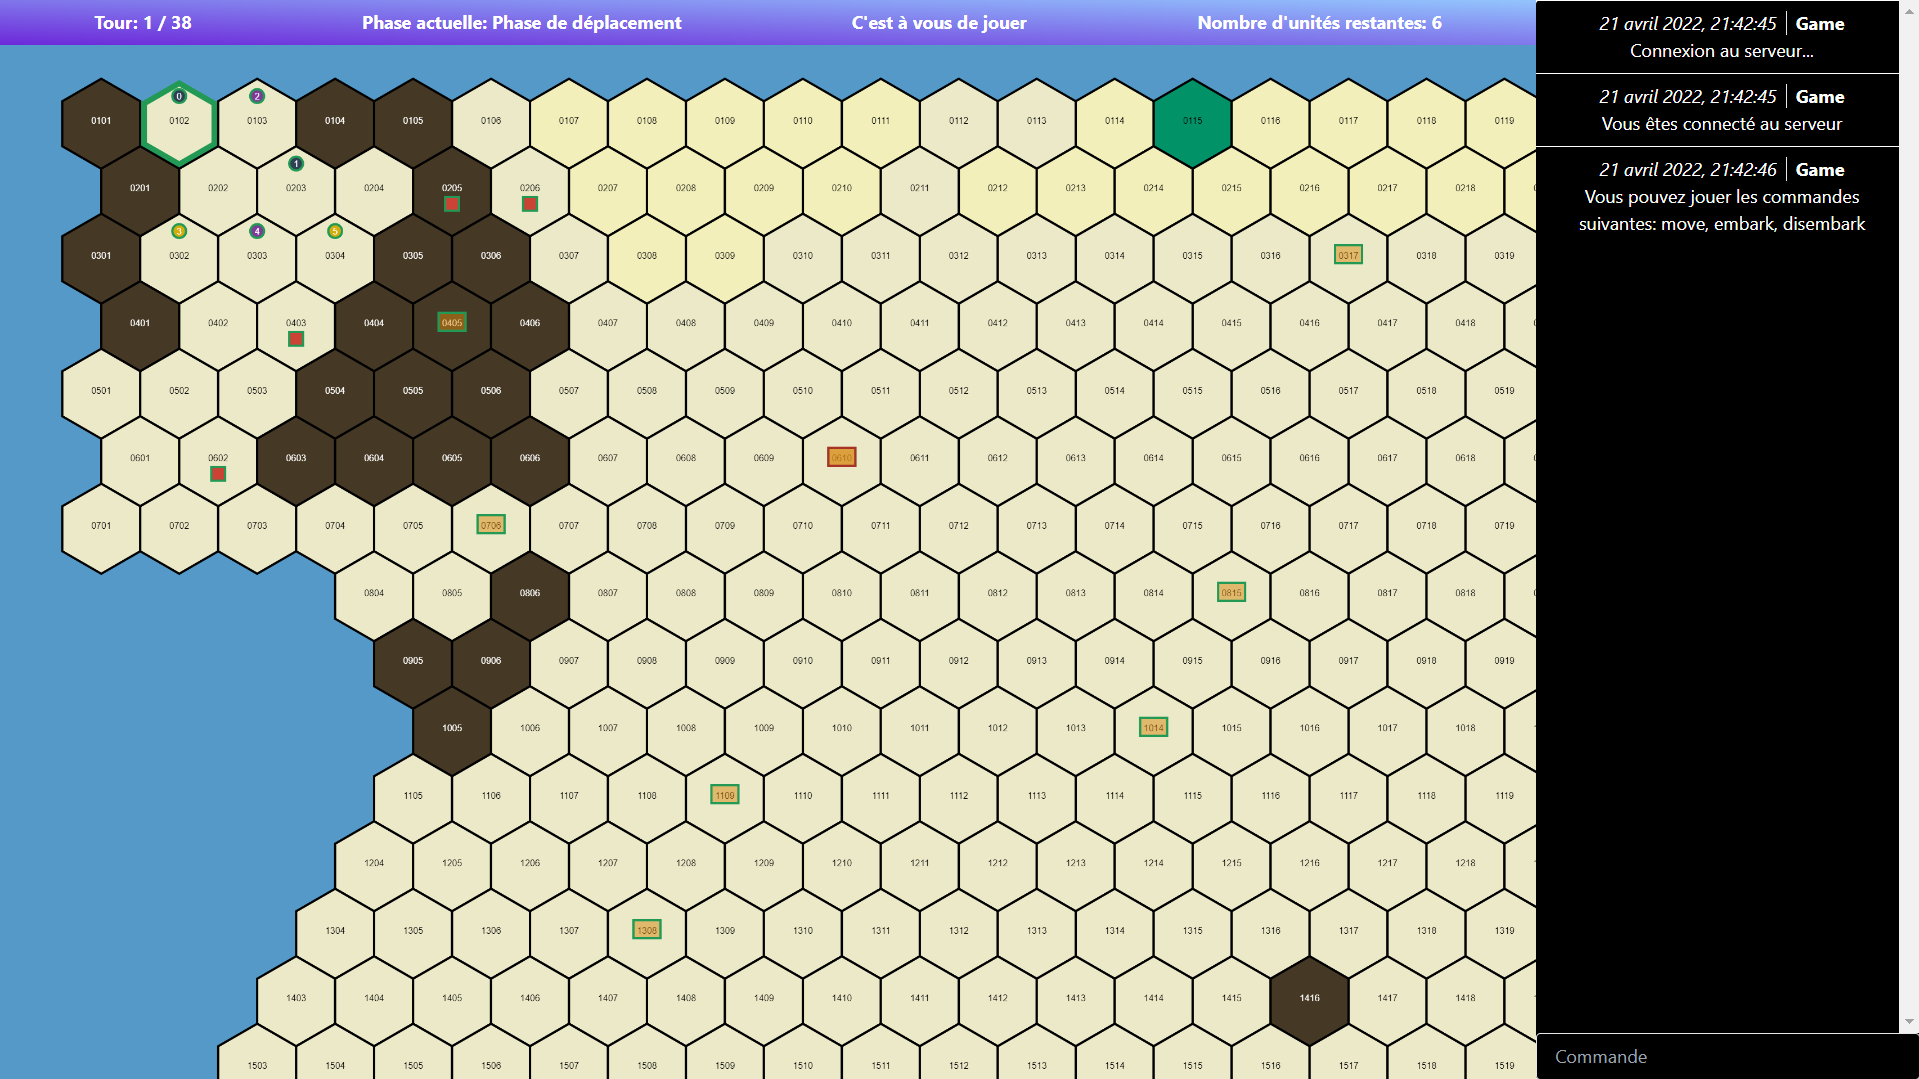
\includegraphics[scale=0.35]{data/plateau_du_jeu.png}
    \caption{Plateau du jeu Desert Fox}.
\end{figure}

En bas de la carte, Nous pouvons observer une légende, en bas à gauche.\\

\begin{figure}[H]
\centering
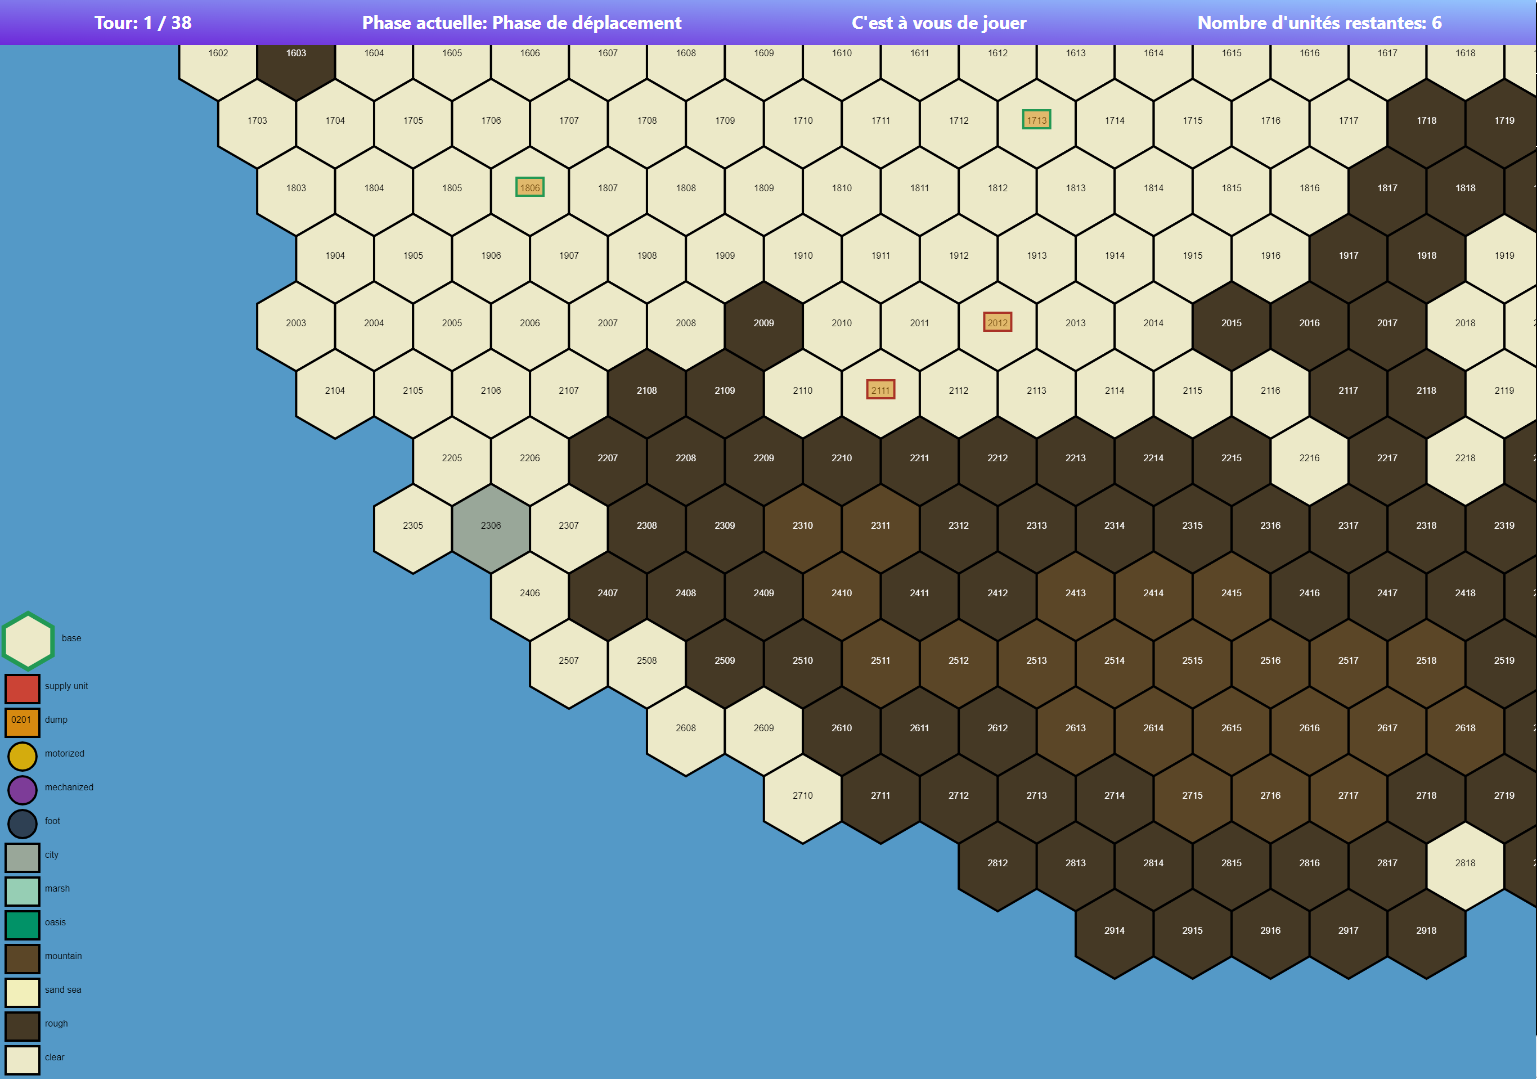
\includegraphics[scale=0.45]{data/Bas_de_map.png}
\caption{Bas de la carte du jeu}.
\end{figure}
\begin{figure}[H]
    \centering
    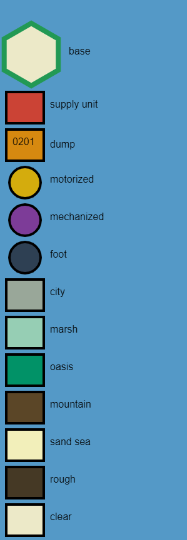
\includegraphics[scale=0.8]{data/Map_Legend.png}
    \caption{Légende de la carte du jeu}.
\end{figure}

Voici la page du joueur 1 qui peut jouer.\\
\begin{figure}[H]
\centering
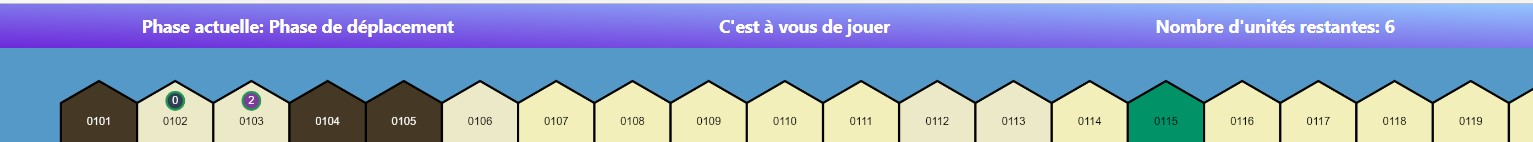
\includegraphics[scale=0.6]{data/player_1_acces.jpg}
\caption{Barre d'information du joueur 1}.
\end{figure}

Voici la page du joueur 2 qui doit attendre l'adversaire de jouer.\\
\begin{figure}[H]
\centering

\includegraphics[scale=0.6]{data/joueur_2.jpg}
\caption{Barre d'information du joueur 2}.
\end{figure}

Le joueur qui peut jouer peut faire bouger son unité dans le terminal a droite de l'image.
Nous pouvons voir que l'unité 0 s'est déplacé de l'hexagone \lstinline{0102} à \lstinline{0206}. Le déplacement est valide car on ne dépasse pas le mouvement alloué de l'unité (MA).\\

\begin{figure}[H]
\centering
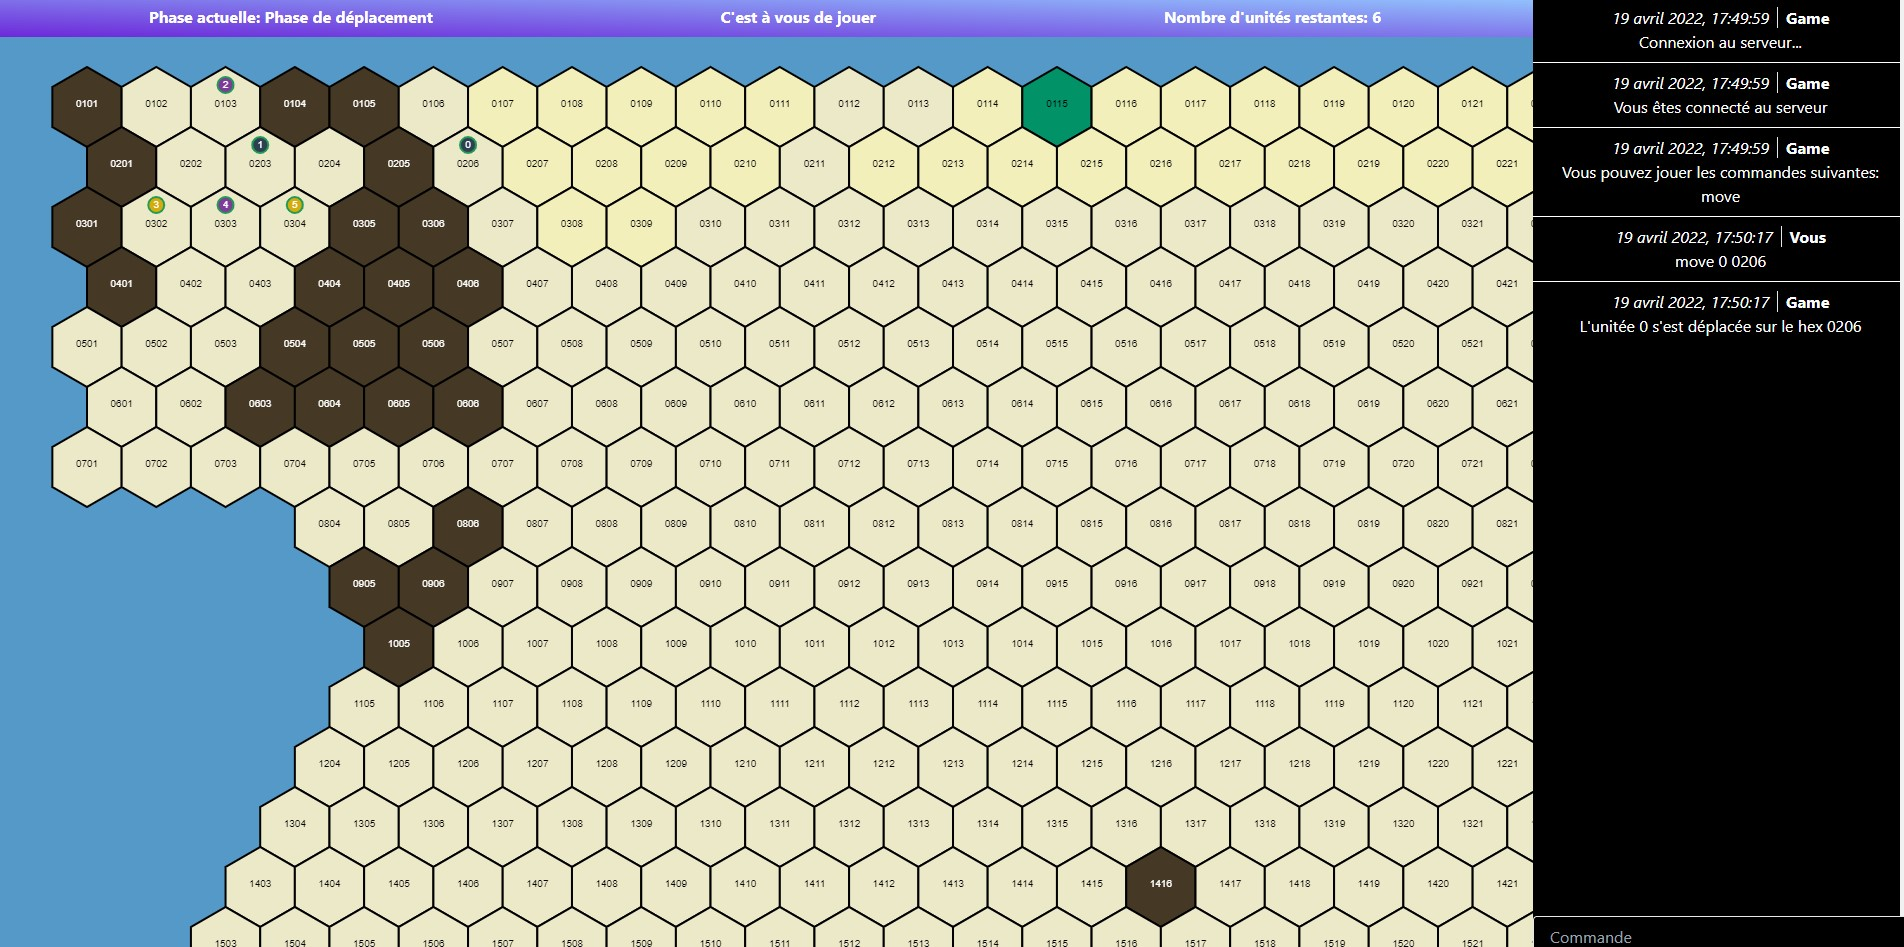
\includegraphics[scale=0.35]{data/move_unit_player_1.jpg}
\caption{Mouvement de l'unité \lstinline{0} vers l'hexagone \lstinline{0206}}.
\end{figure}

Le joueur peut aussi utiliser une de ses unités de soutien pour bouger soit une unité de type {\tt foot} soit un dump.
Il peut faire cela avec la commande {\tt embark} qui prend en parametre l'identifiant de l'unité du soutien qui va embarquer, ainsi que l'identifiant de l'unité qui va etre embarquée. Voici un exemple :\\

\begin{figure}[H]
    \centering
    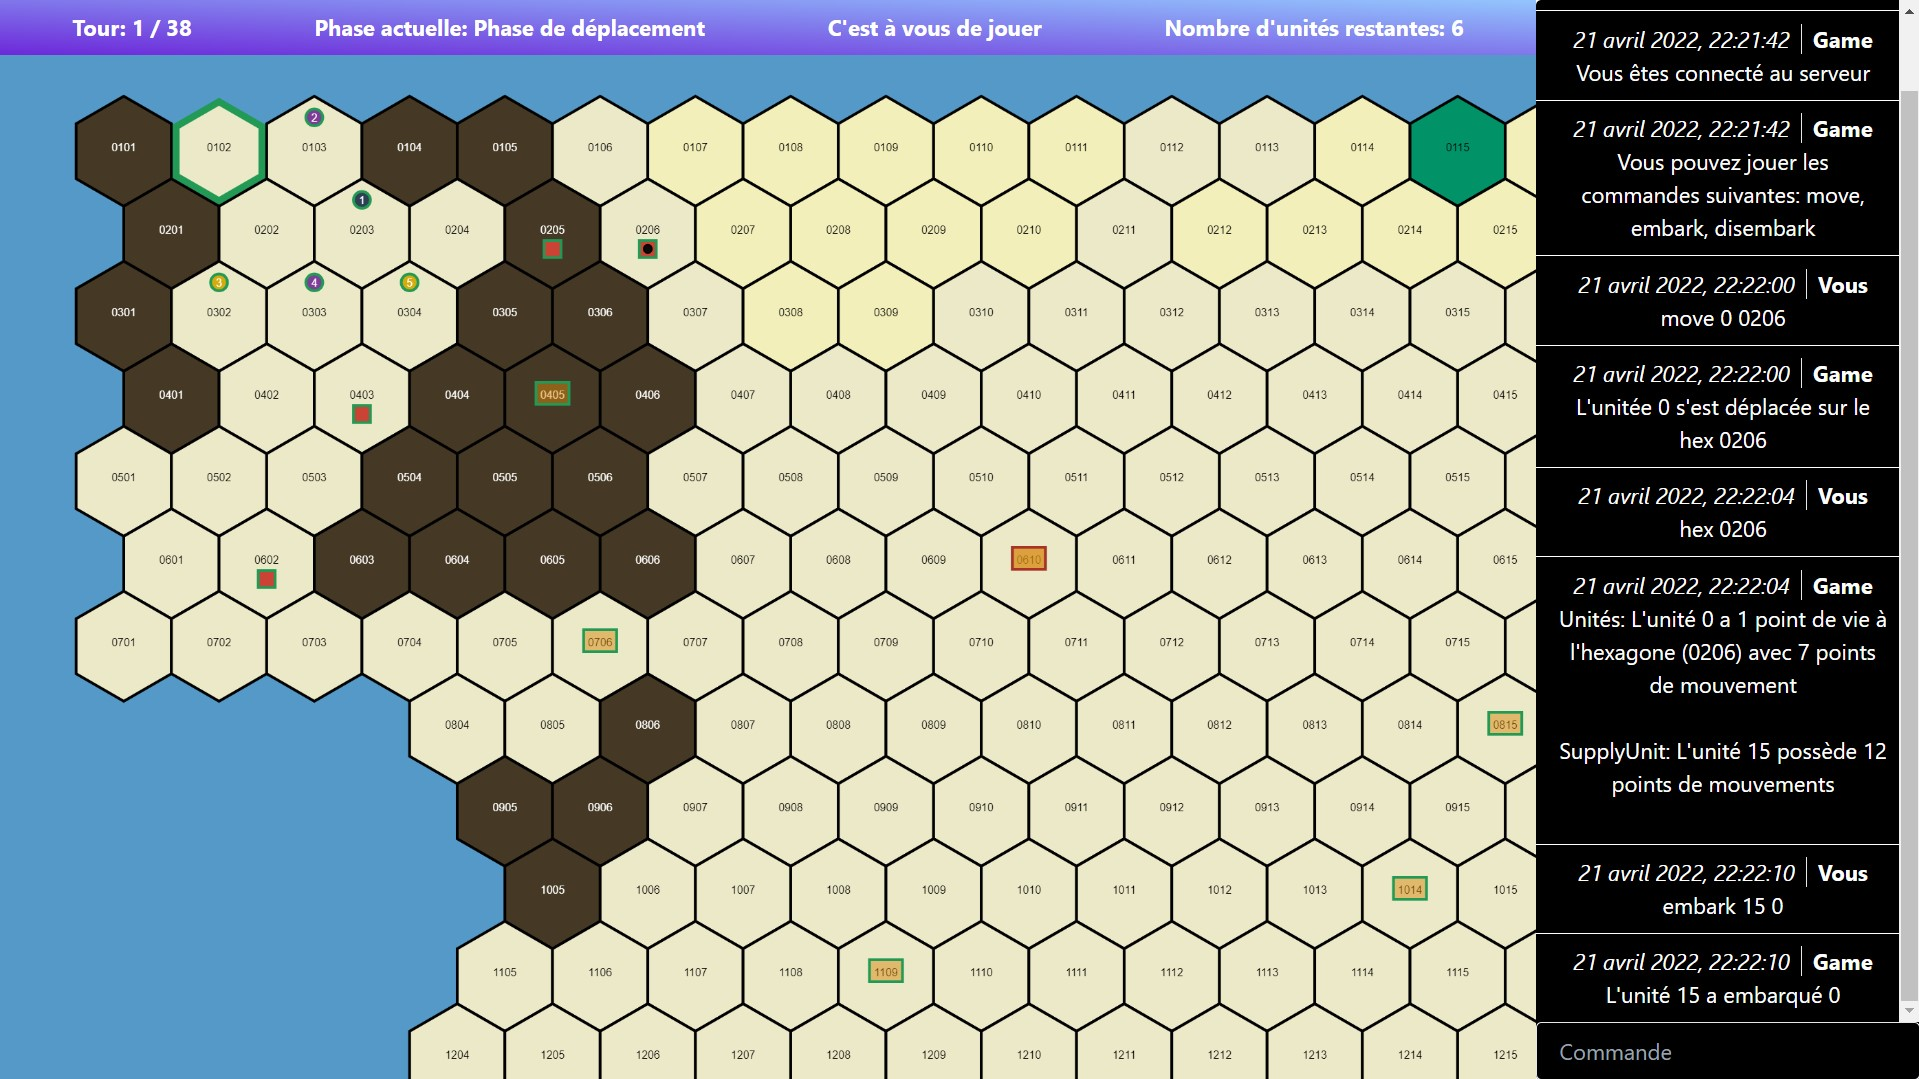
\includegraphics[scale=0.35]{data/Embark_command.jpg}
    \caption{Embarquement de l'unité \lstinline{0} dans l'unité de soutien  \lstinline{15}}.
\end{figure}

Il faut noter que l'unité qui est embarqué est inexistante dans la carte. Elle ne peut donc pas bouger elle meme, ni attaquer. Si l'unité du soutien a embarqué une unité, elle bougera avec elle. Dans la figure ci dessous nous pouvons voir que si nous embarquons un dump, qui est une entité qui ne peut pas bouger elle meme, nous pouvons la faire bouger avec l'unité de soutien. Ici nous la bougeons de l'hexagone \lstinline{0406} vers l'hexagone \lstinline{0407} \\

\begin{figure}[H]
    \centering
    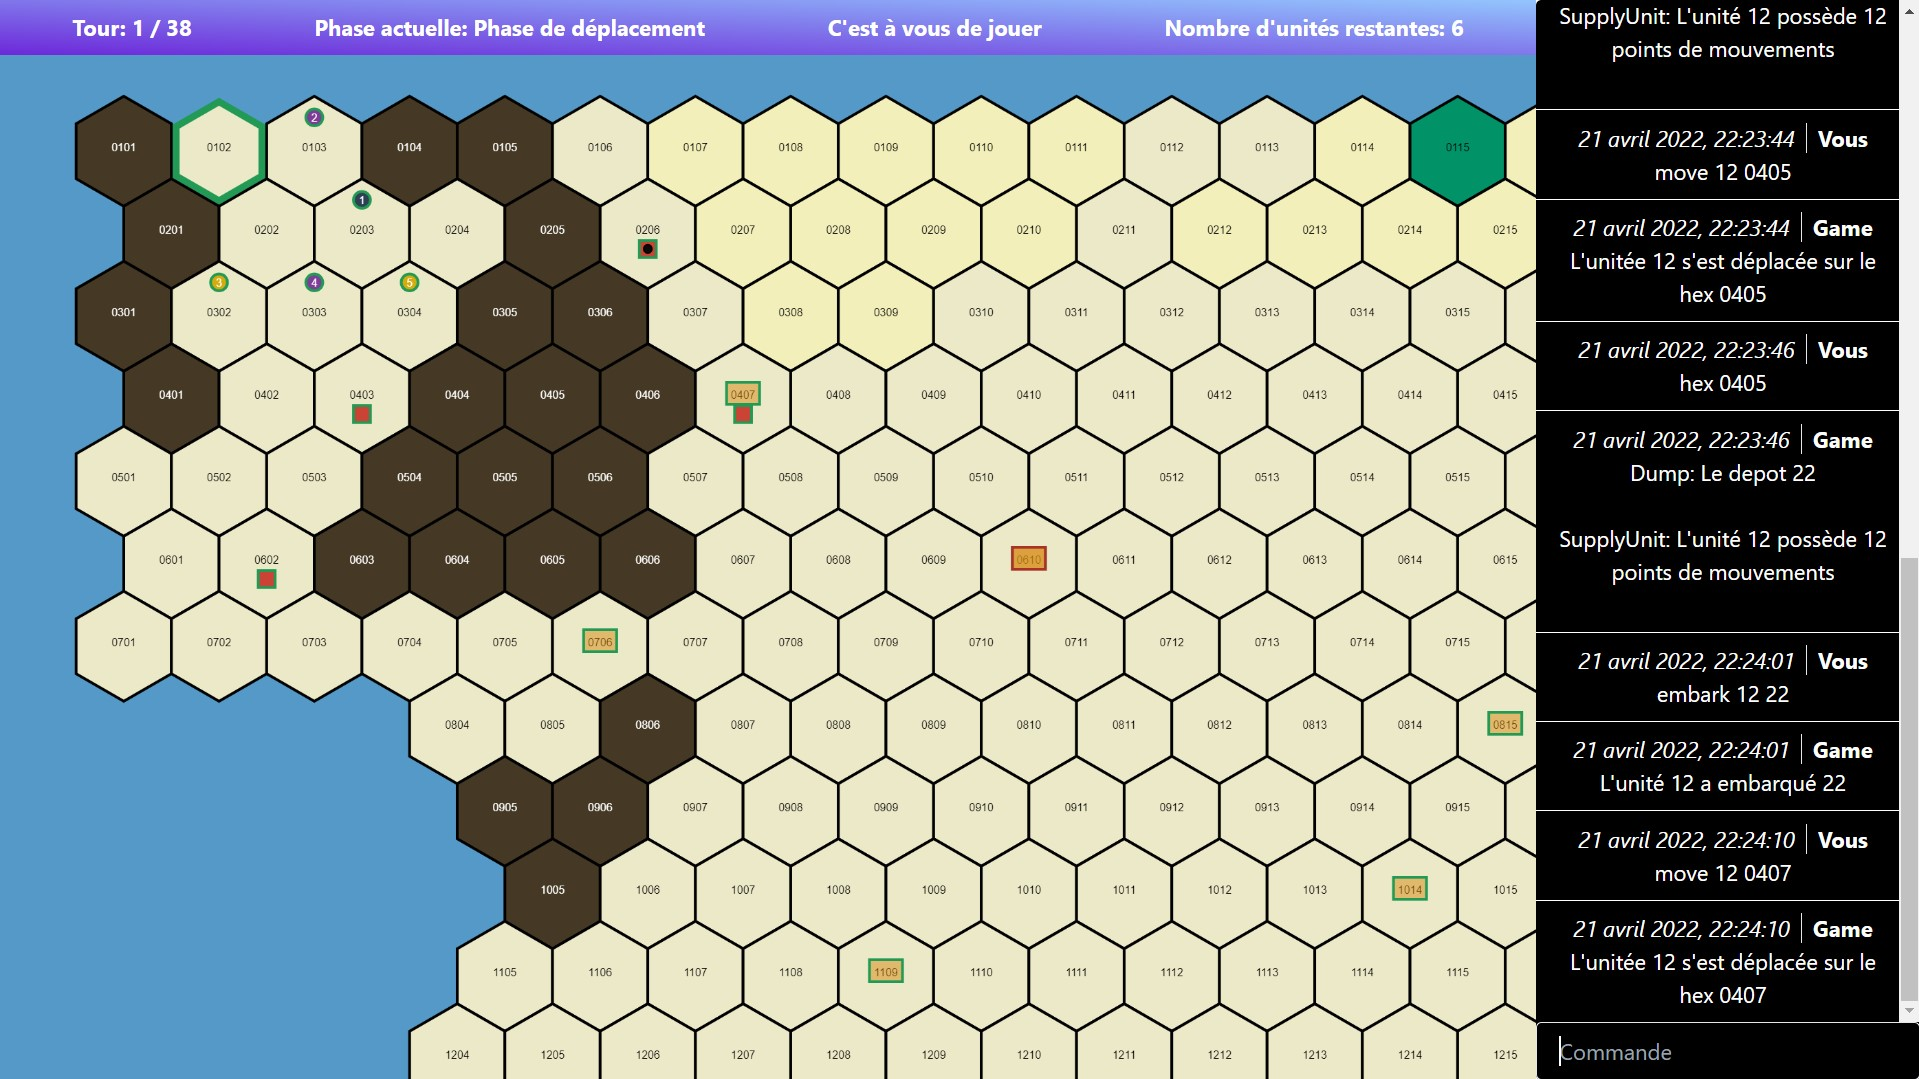
\includegraphics[scale=0.35]{data/Embark_dump.jpg}
    \caption{Embarquement du dump \lstinline{22} dans l'unité de soutien  \lstinline{12} suivi par un deplacement de l'unité du soutien à l'hexagone \lstinline{0407} (avec le dump)}.
\end{figure}

Afin de pouvoir reutiliser l'unité ou l'entité embarquée, nous devons utiliser la commande disembark, laquelle permet de debarquer cette dernière.
Dans la figure ci dessous nous pouvons voir que apres avoir bougé l'unité de soutien {\tt 15}, laquelle contient l'unité {\tt 0} et désembarquer, l'unité est dorénavant disponible pour un autre mouvement ou action. Elle est aussi affiché à nouveau dans la carte.\\

\begin{figure}[H]
    \centering
    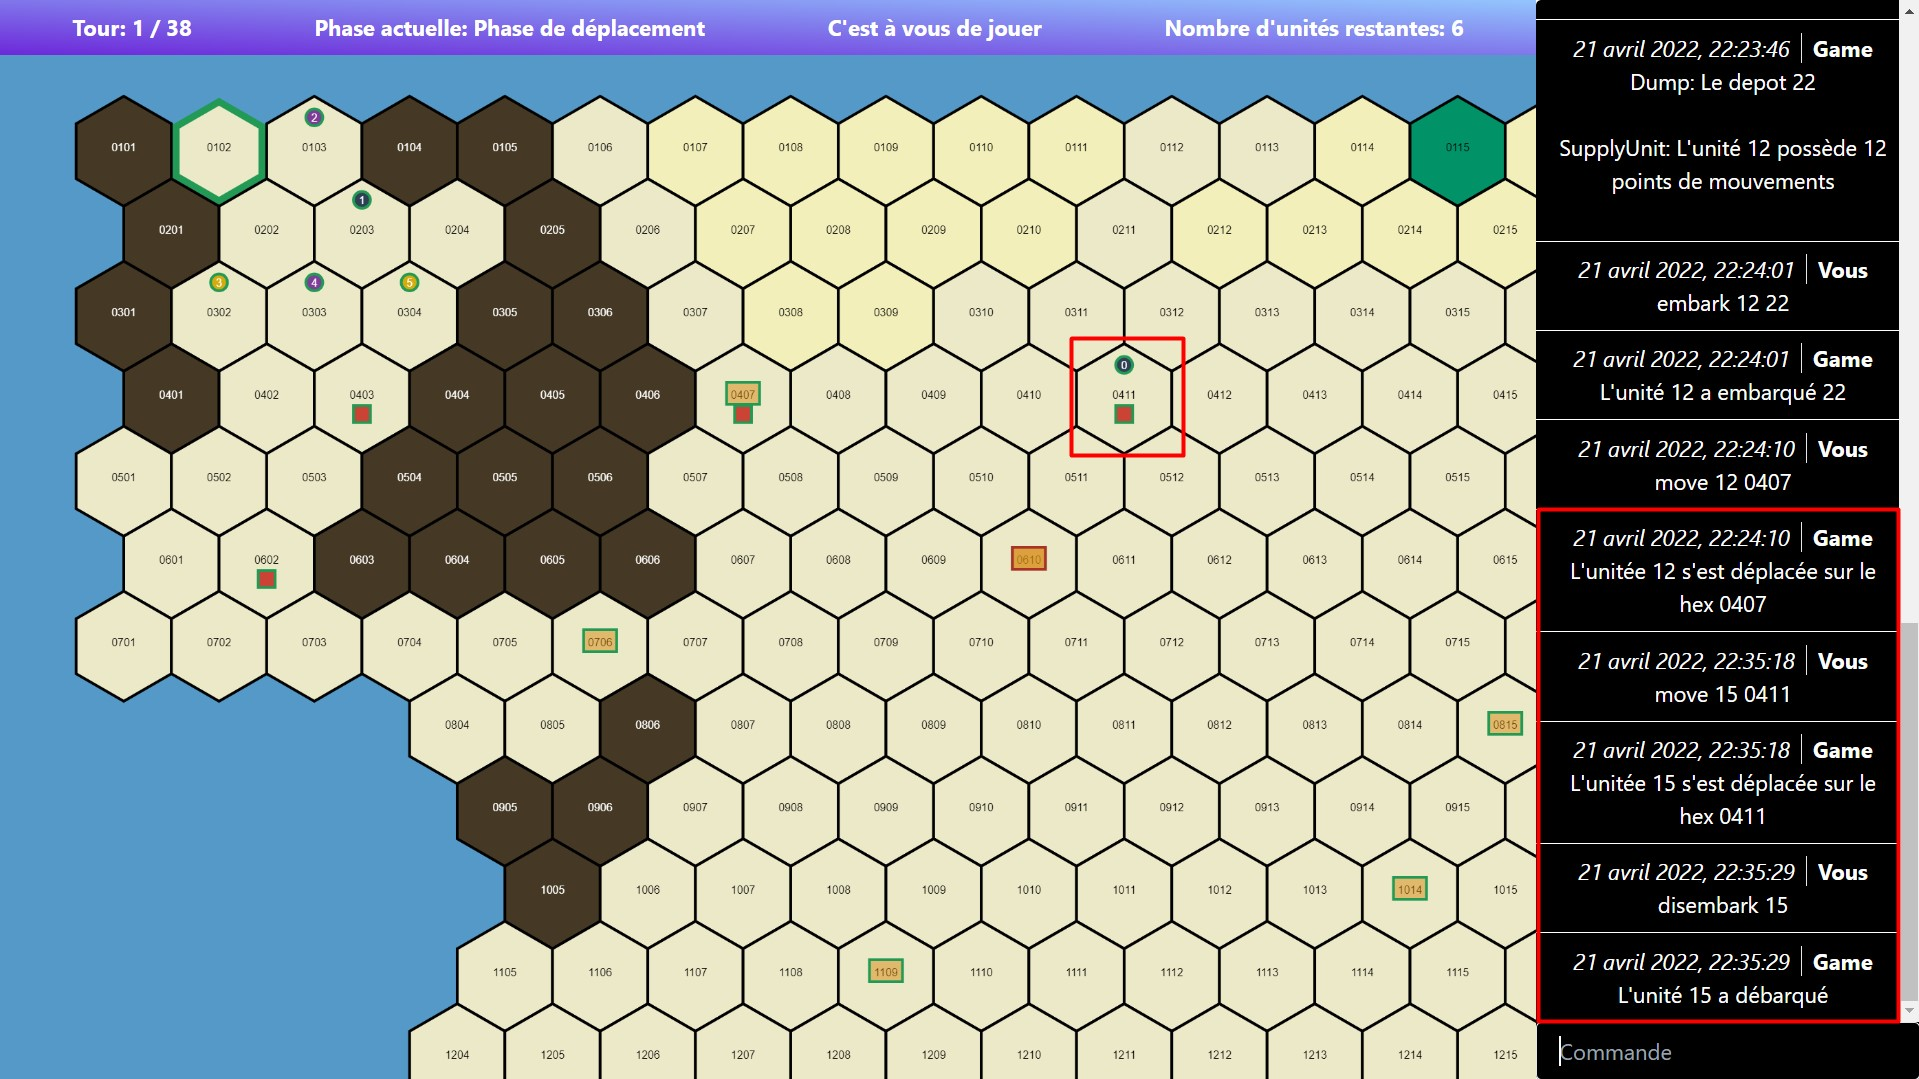
\includegraphics[scale=0.35]{data/Disembark.jpg}
    \caption{Mouvement de l'unité du soutien \lstinline{15}, laquelle contient l'unité \lstinline{0} à l'hexagone \lstinline{0411}, suivi du désembarquement de l'unité embarquée}.
\end{figure}

L'utilisateur peut aussi utiliser la commande {\tt attack} pour attaquer une unité adverse. Il faut noter que l'attaque est uniquement possible si l'unité est dans une case adjacente de l'unité adverse. Dans l'exemple ci dessous, nous pouvons voir que l'unité {\tt 5} \\

Le joueur peut afficher des informations concernant ses unités dans le terminal.
En tapant \og units \fg{}, le joueur à toutes ses unités présent avec le mouvement point et  les points de vies.\\
\begin{figure}[H]
\centering
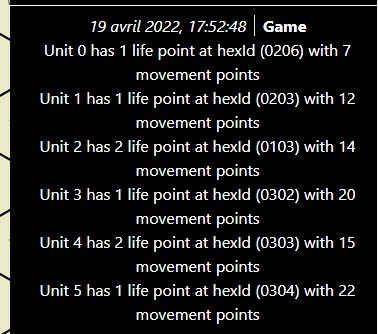
\includegraphics[scale=0.6]{data/info_units.jpg}
\caption{Terminal qui donne les informations des unités du joueur 1 }.
\end{figure}

Quand le joueur a terminé son tour, il doit écrire dans le terminal \og done \fg{}
le joueur ne pourra que communiquer par chat à l'adversaire et l'adversaire peuvent continuer à jouer.\\
\begin{figure}[H]
\centering
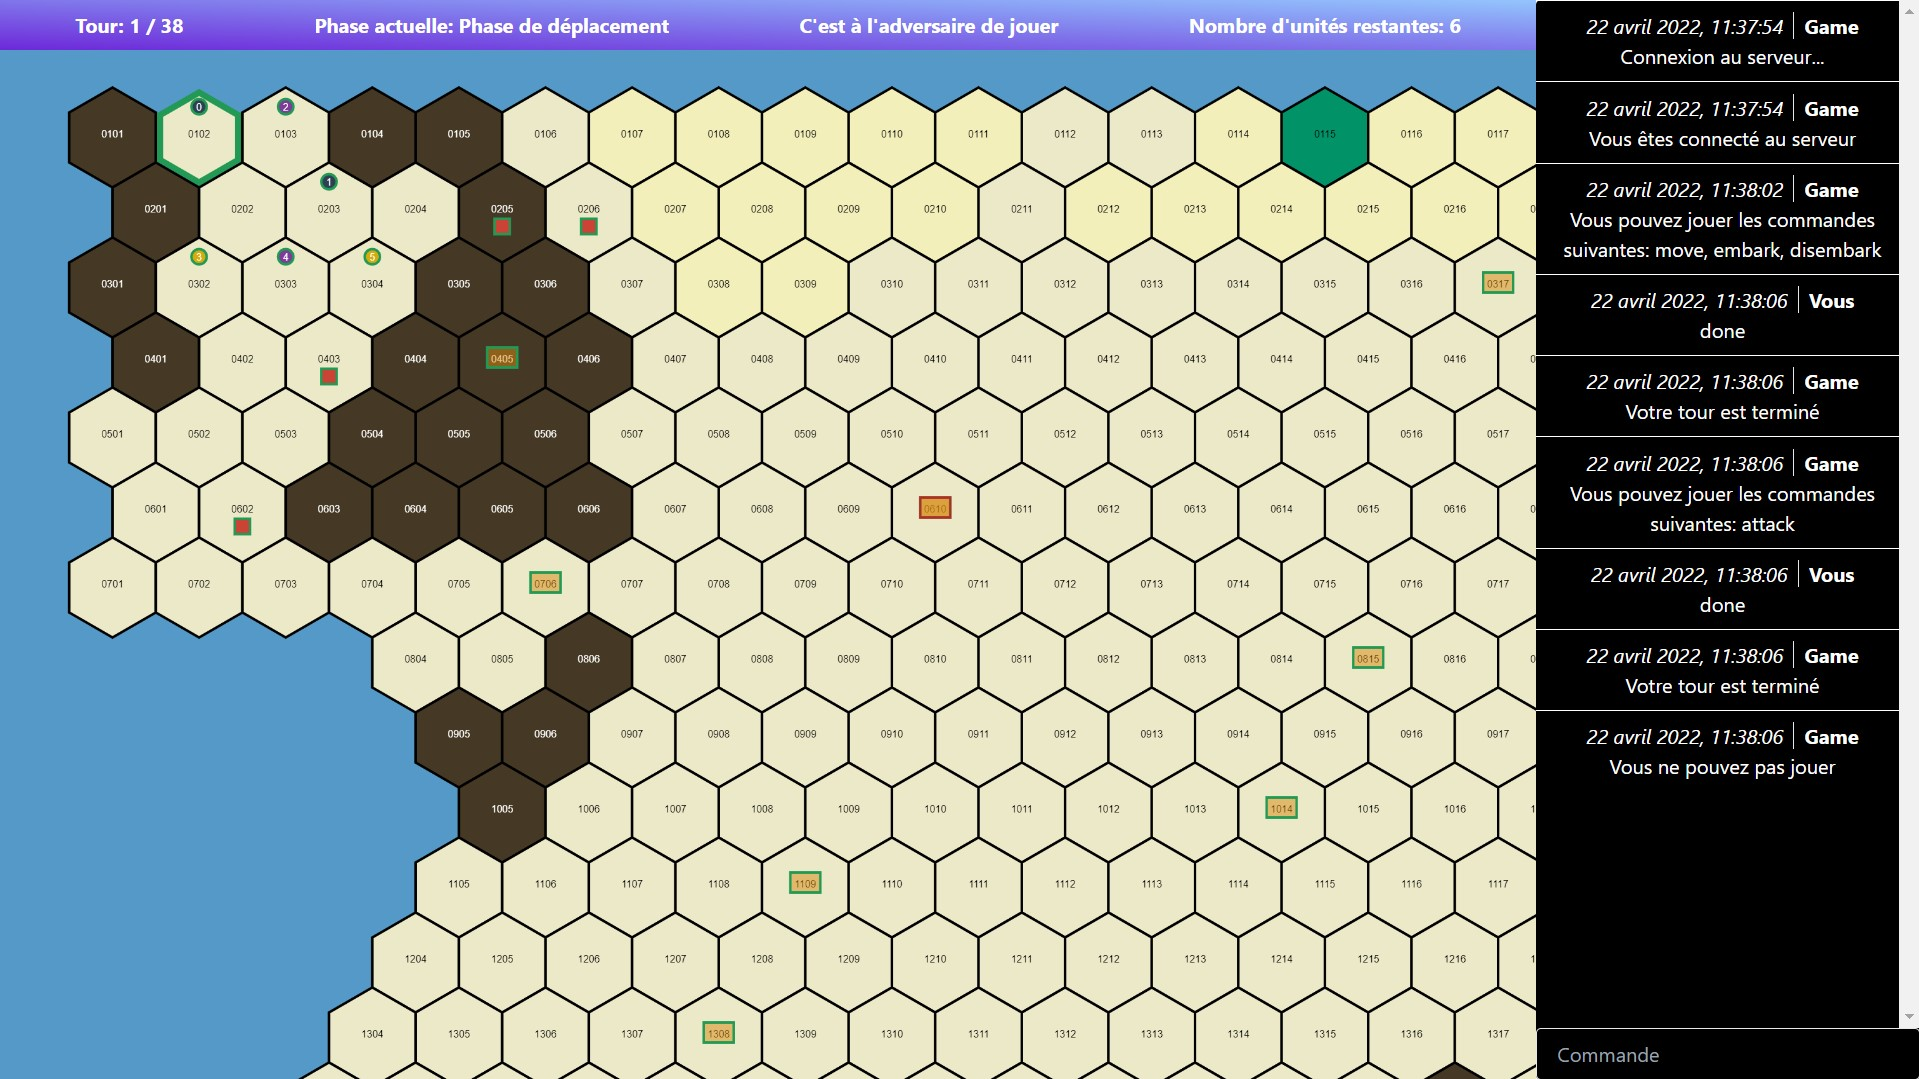
\includegraphics[scale=0.35]{data/fin_tour.jpg}
\caption{Fin du tour pour le joueur 1}.
\end{figure}


Le joueur peut aussi aficher les entités, par exemple les unités, les bases, les dumps et les unités de soutien qui sont present dans une hexagone. 
Cela est possible grace a la commande {\tt hex}, qui prend en parametre un identifiant d'hexagone.Voici un exemple :\\

\begin{figure}[H]
    \centering
    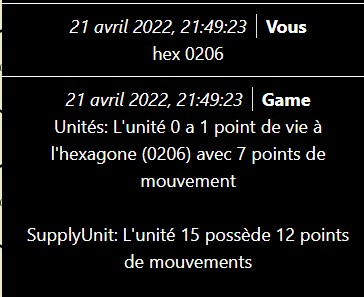
\includegraphics[scale=0.75]{data/hex_command.jpg}
    \caption{Utilisation de la commande hex}.
\end{figure}

Les deux joueurs peuvent communiquer ensemble  à l'aide du terminal, le joueur doit écrire au dans le terminal \og message \fg{} puis écrit son message.\\
\begin{figure}[H]
\centering
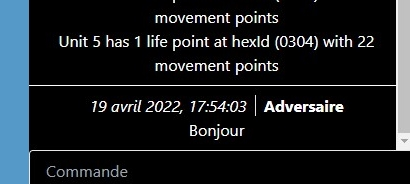
\includegraphics[scale=0.6]{data/chat.jpg}
\caption{Communication entre deux joueurs}.
\end{figure}

Un message d'erreur s'affiche dans le terminal si le joueur écrit  des mauvaises commandes.
Par exemple, le joueur oublie les arguments, ou donne un mauvais hexagone.\\

\begin{figure}[H]
\centering
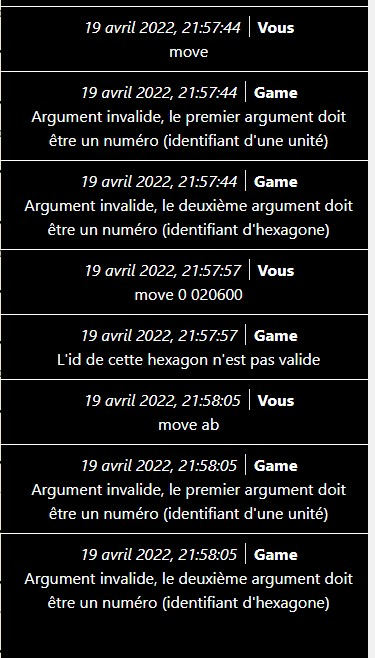
\includegraphics[scale=0.6]{data/erreur.jpg}
\caption{Exemple de mauvaises commandes}.
\end{figure}

